\documentclass{article}
\usepackage[utf8]{inputenc}
\usepackage[margin=1in]{geometry}
\usepackage{amsmath}
\usepackage{amssymb}
\usepackage{listings}
\usepackage{graphicx}
\usepackage{float}

\graphicspath{{images/}}

\title{Solutions to the Assignment - 2 : CS5480 - \\
Deep Learning}
\author{Vishwak Srinivasan\\
\texttt{CS15BTECH11043}}
\date{}

\begin{document}
\maketitle

\section*{Question 1}
\subsection*{Part a}
\begin{flushleft}
The code for the neural net in available in the file \texttt{Question1.py}. The instructions for running this code can be obtained by running \texttt{python3 Question1.py -h}. Single string help statements have been provided, and default values have been shown.

A check for correctness of the program specified in the problem was to try a full-batch gradient descent algorithm for the loss function. As expected, the loss decreased monotonically. The graph of this variation is shown below:
\begin{figure}[H]
\centering
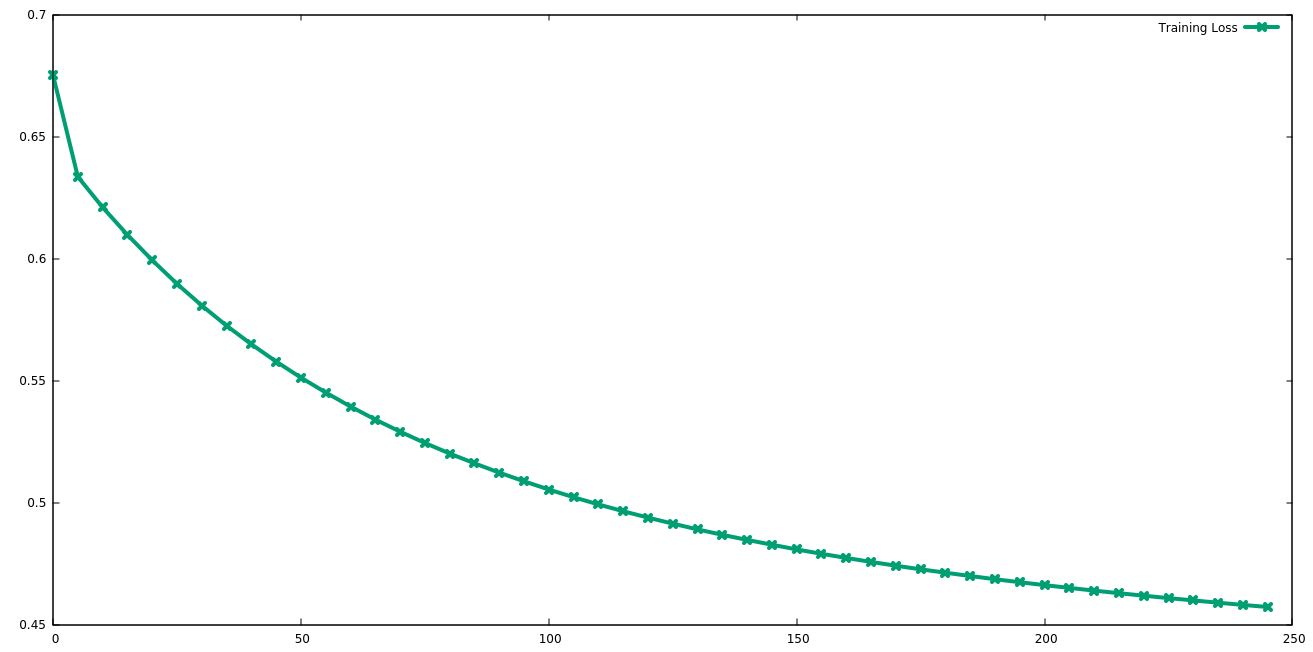
\includegraphics[width=0.7\linewidth]{train_full_batch_q1.png}
\end{figure}
\end{flushleft}

\subsection*{Part b}
\begin{flushleft}
This baseline accuracy is implemented in the results section of the code. To make an proper random guess, it is important to know the class-(im)balance in the output labels. I calculate these probabilities and create a tensor of the length of the targets and initialize using \texttt{torch.bernoulli(p=<calculated probability>)}. Lines of interest in the script are L169-L178 and L192-L201.
\end{flushleft}

\subsection*{Part c}
\begin{flushleft}
I used a constant learning rate schedule. For the specifications of this problem i.e., \texttt{batch\_size} = 100, \texttt{H} = 5, the best learning rate I could get is 0.008 (chosen from a set \(\{0.0001, \ldots, 0.0009, 0.001, \ldots, 0.009, 0.01, \ldots, 0.05 \}\)). The random state is saved in \texttt{random-state.pt} for reproducibility. I trained it until the training classification error increased considerably per epoch (``jumping from an otherwise stable point") or didn't decrease considerably per epoch (reaching a ``local minimum"), which in this case was 96 epochs. The training set accuracy achieved after 96 epochs was \(92.91\%\) and the testing set accuracy achieved after 96 epochs was \(93.99\%\). Below are the graphs of the variations observed (L: Train, R: Test):
\begin{figure}[H]
\begin{minipage}{0.49\linewidth}
\centering
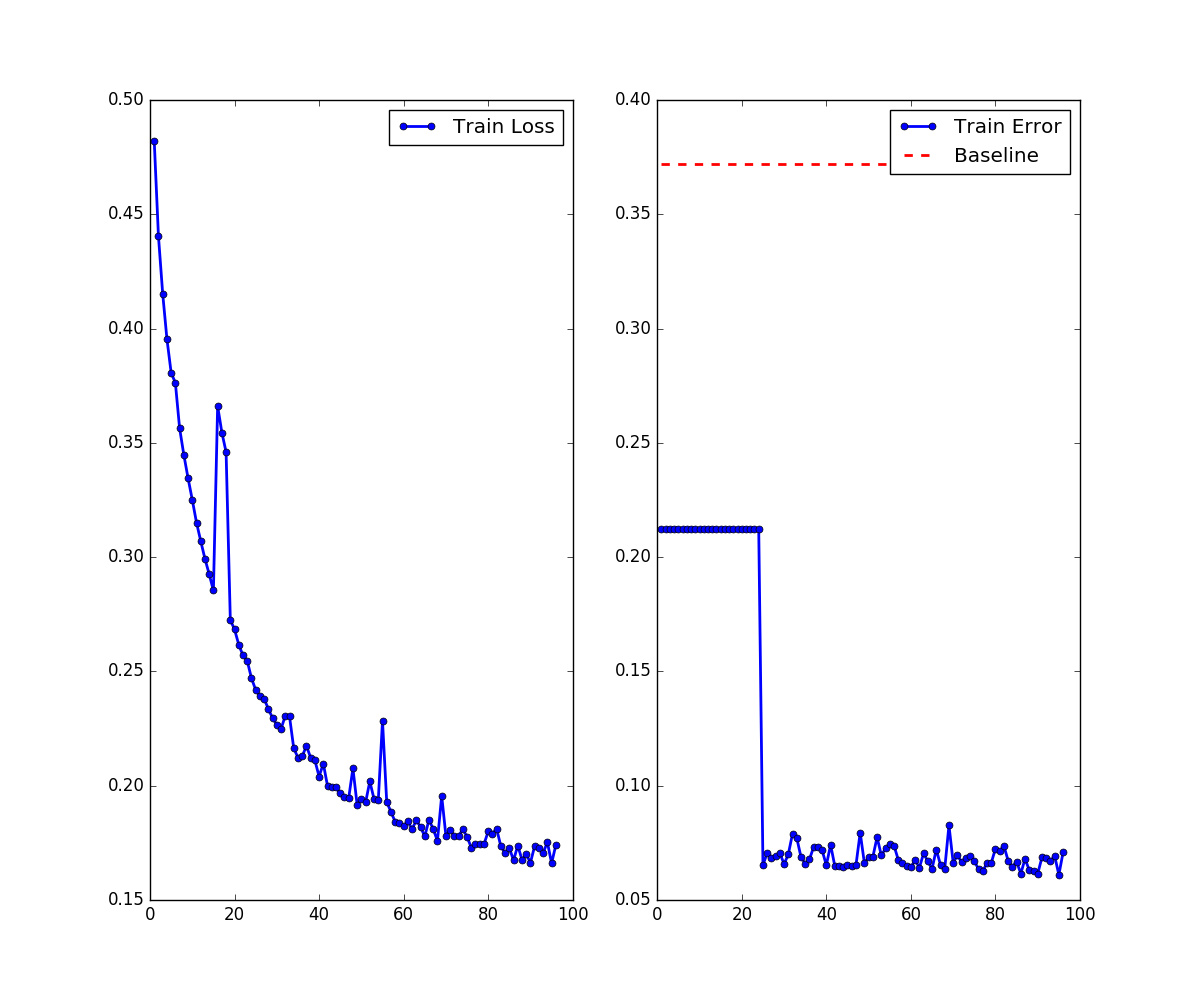
\includegraphics[width=0.95\textwidth]{Train-Statistics-sgd-batchsize=100-bce.png}
\end{minipage}
\hfill
\begin{minipage}{0.49\linewidth}
\centering
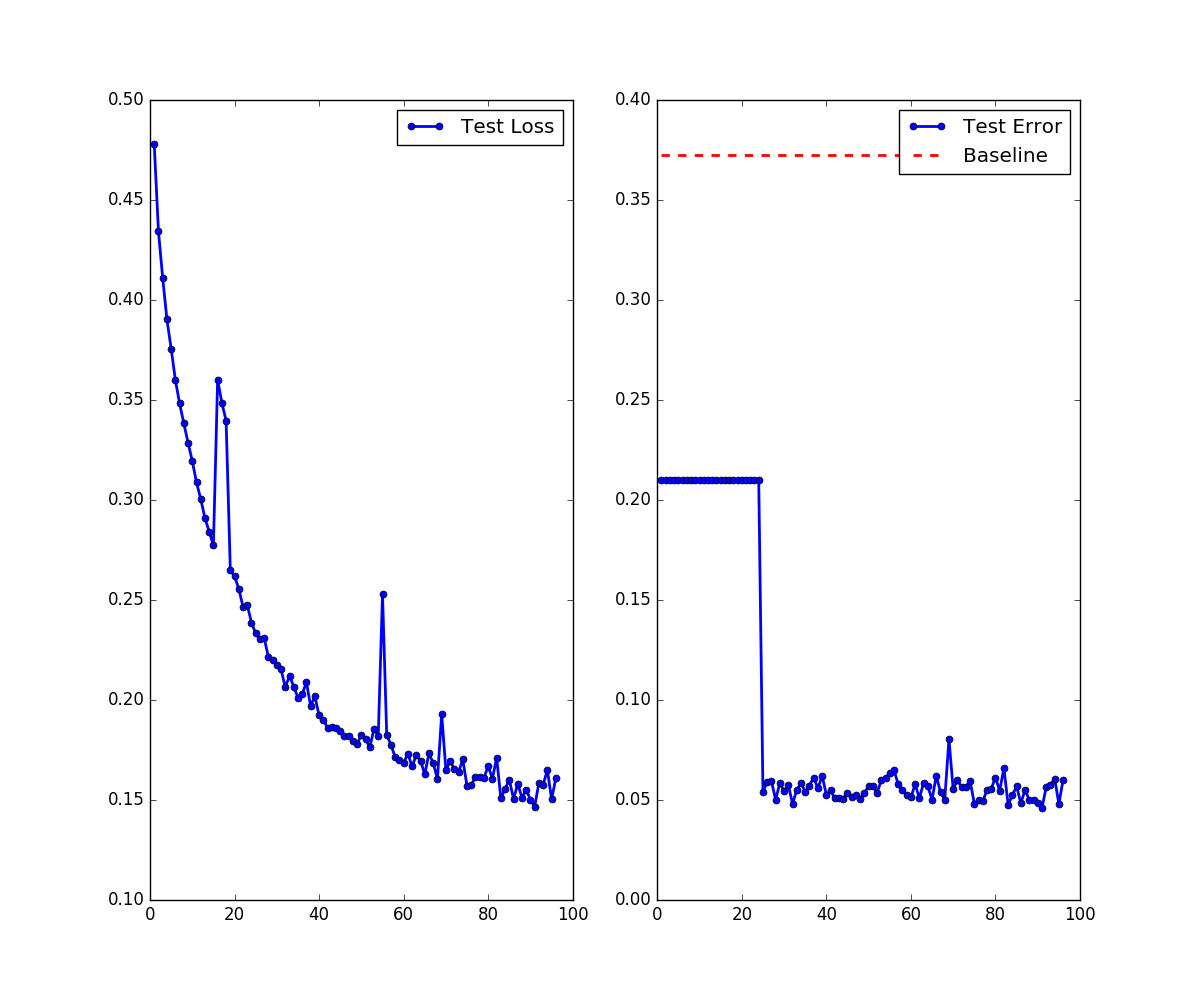
\includegraphics[width=0.95\textwidth]{Test-Statistics-sgd-batchsize=100-bce.png}
\end{minipage}
\end{figure}
\end{flushleft}

\subsection*{Part d}
\begin{flushleft}
Clearly, for the same learning rate and the same number of epochs, it would be hard to view similar performance. Hence, I change the learning rate (to 0.01) and train the network for a bit longer (2000 epochs). The final results after 96 iterations and the end of the training are reported below:
\begin{center}
\begin{tabular}{|c|c|c|}
\hline
& Train Accuracy & Test Accuracy \\
\hline
96 epochs & \(\approx 78\%\) & \(\approx 79\%\) \\
\hline
2000 epochs & \(93.11\%\) & \(94.27\%\) \\
\hline
\end{tabular}
\end{center}

The variation graph is shown below (L: Train, R: Test):
\begin{figure}[H]
\begin{minipage}{0.49\linewidth}
\centering
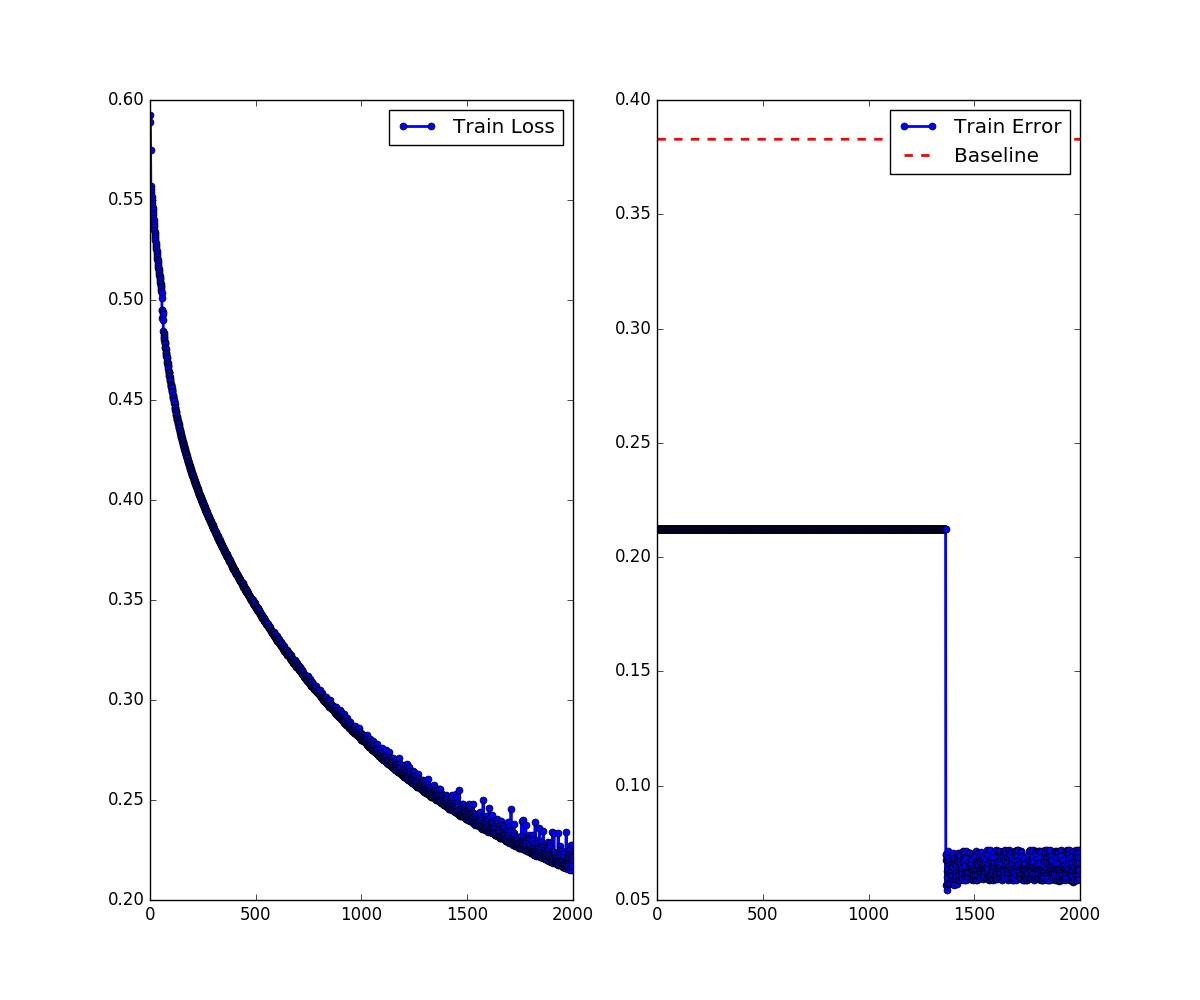
\includegraphics[width=0.95\textwidth]{Train-Statistics-sgd-batchsize=8143-bce.png}
\end{minipage}
\hfill
\begin{minipage}{0.49\linewidth}
\centering
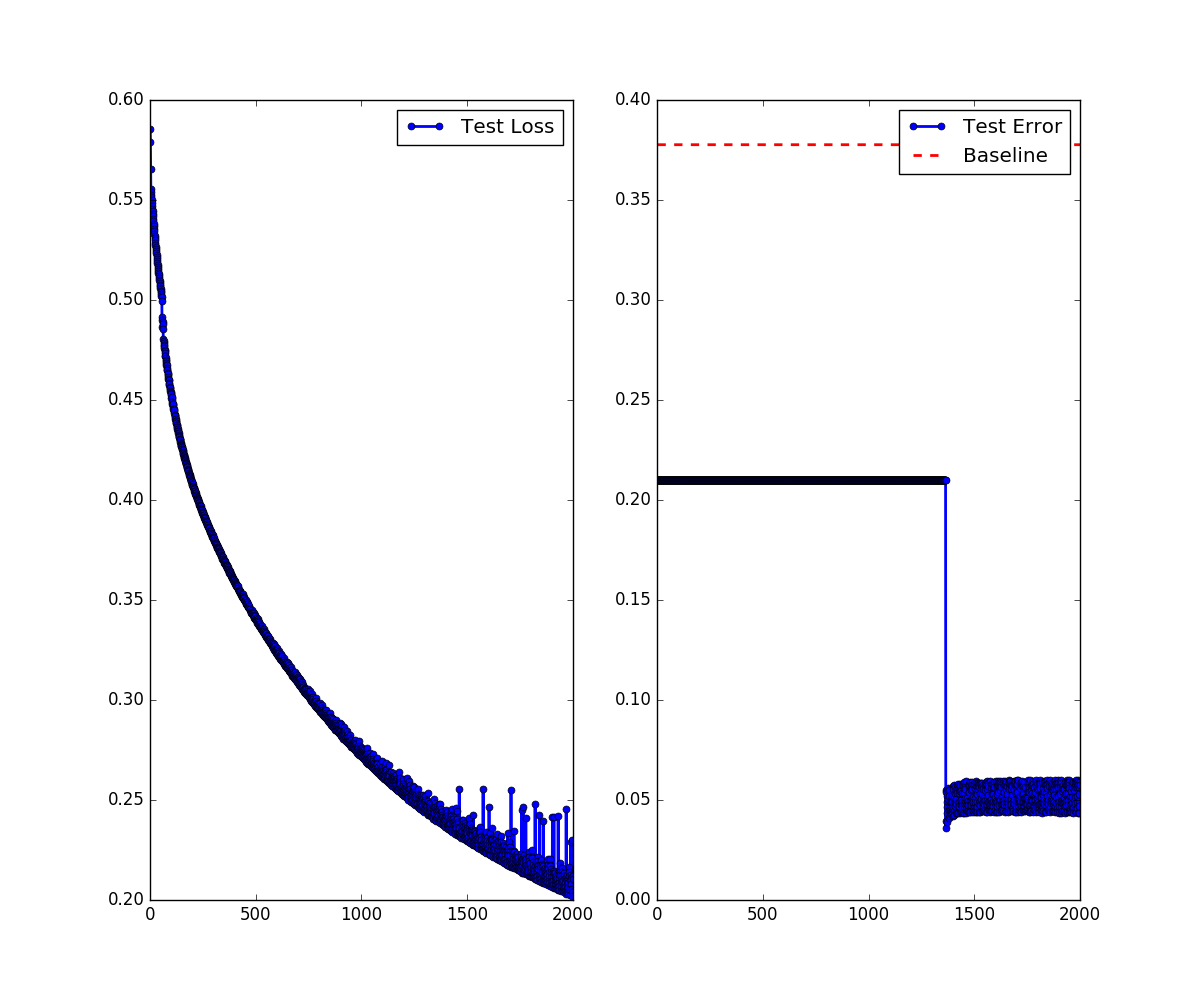
\includegraphics[width=0.95\textwidth]{Test-Statistics-sgd-batchsize=8143-bce.png}
\end{minipage}
\end{figure}
\end{flushleft}

\subsection*{Part e}
\begin{flushleft}
I use Adam as the learning algorithm for this sub-problem. The global learning rate in Adam is set to \(3 \times 10^{-4}\) (following Andrej Karpathy's claim), and the bias correction parameters are set to the default values. The stopping epochs for the 5 different configurations and the end performance are tabulated below:
\begin{center}
\begin{tabular}{|c|c|c|c|}
\hline
H & Stopping Epochs & Training Set Accuracy & Testing Set Accuracy \\
\hline
1 & 55 & \(\approx 78.6\%\) & \(\approx 79.1\%\)\\
\hline
2 & 350 & \(\approx 98.8\%\)& \(\approx 99.0\%\)\\
\hline
5 & 110 & \(\approx 98.8\%\)& \(\approx 99.1\%\)\\
\hline
10 & 90 & \(\approx 98.8\%\)& \(\approx 99.1\%\)\\
\hline
20 & 70 & \(\approx 98.8\%\)& \(\approx 99.2\%\)\\
\hline
\end{tabular}
\end{center}

Graphically, the variation is shown below (L: Train, R: Test):
\begin{minipage}{0.49\linewidth}
\begin{figure}[H]
\centering
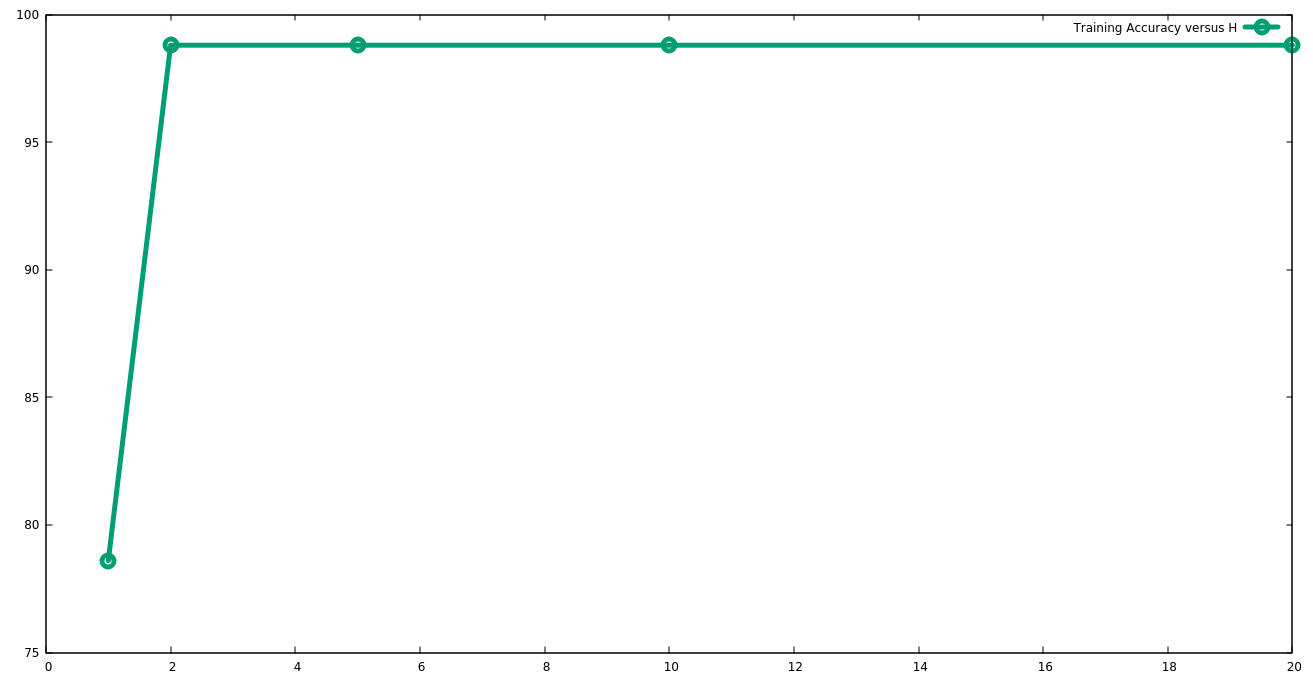
\includegraphics[width=0.95\textwidth]{train_H_BCE.png}
\end{figure}
\end{minipage}
\hfill
\begin{minipage}{0.49\linewidth}
\begin{figure}[H]
\centering
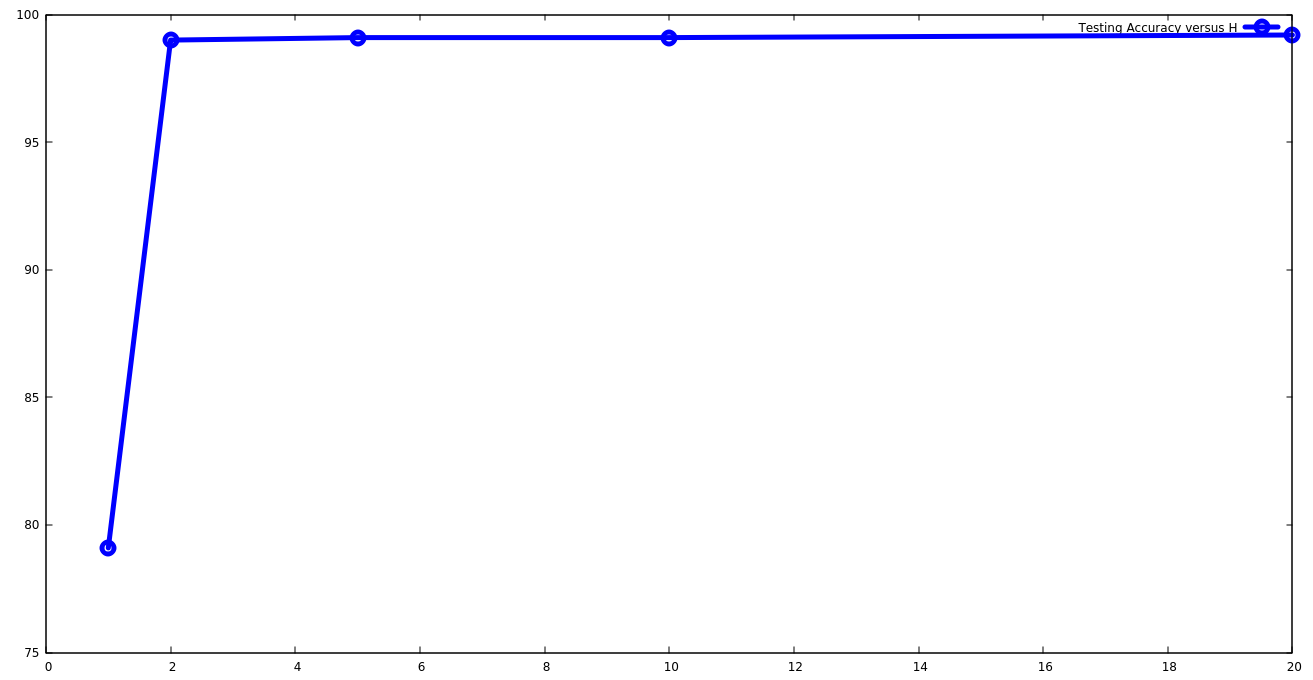
\includegraphics[width=0.95\textwidth]{test_H_BCE.png}
\end{figure}
\end{minipage}
\end{flushleft}

\subsection*{Part f}
\begin{flushleft}
The optimal learning chosen from the same set of specified above is 0.008. The training set accuracy achieved after 70 epochs was \(95\%\) and the testing set accuracy achieved after 70 epochs was \(\approx 96.1\%\). Below are the graphs of the variations observed (L: Train, R: Test):
\begin{figure}[H]
\begin{minipage}{0.49\linewidth}
\centering
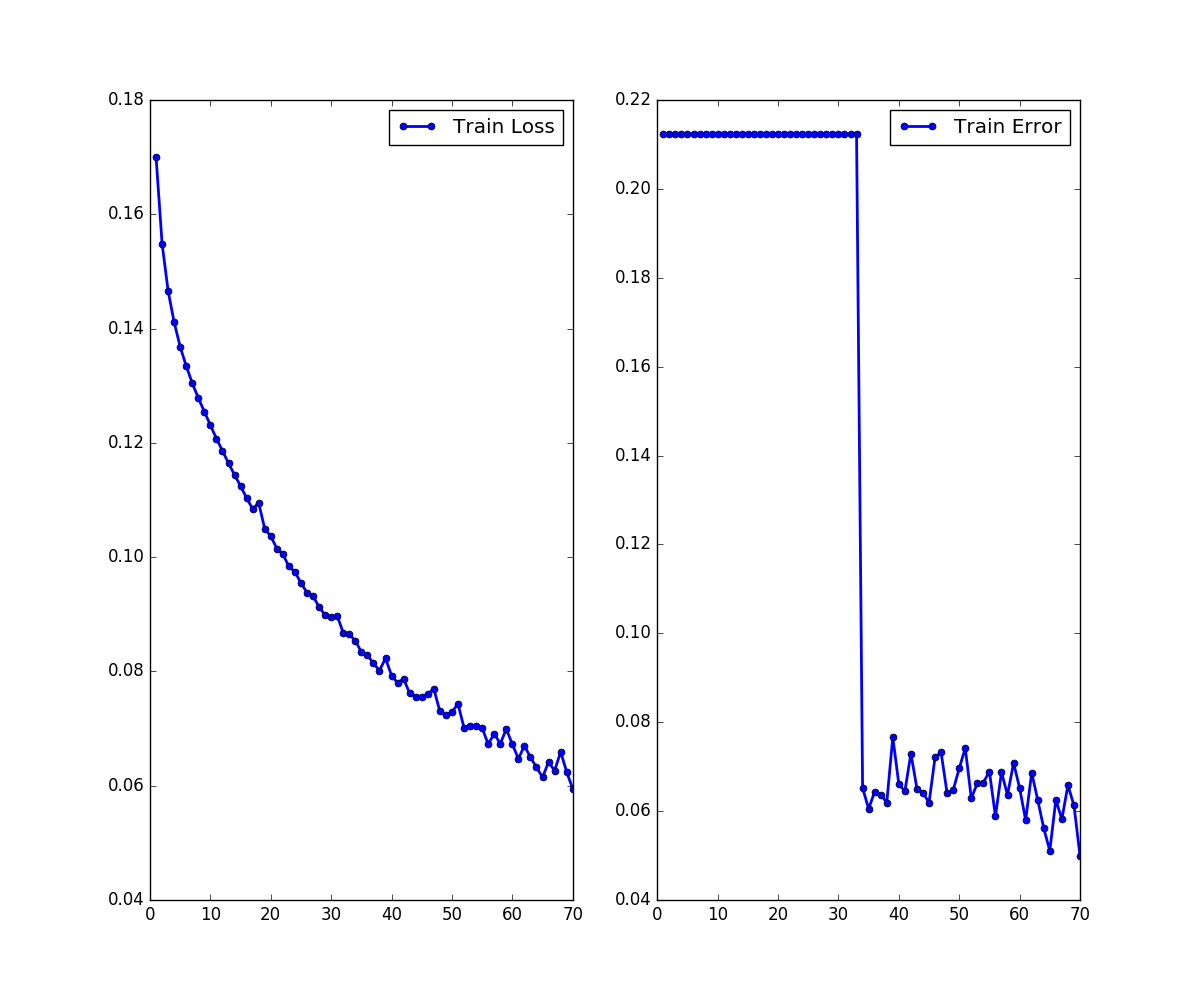
\includegraphics[width=0.95\textwidth]{Train-Statistics-sgd-batchsize=100-mse.png}
\end{minipage}
\hfill
\begin{minipage}{0.49\linewidth}
\centering
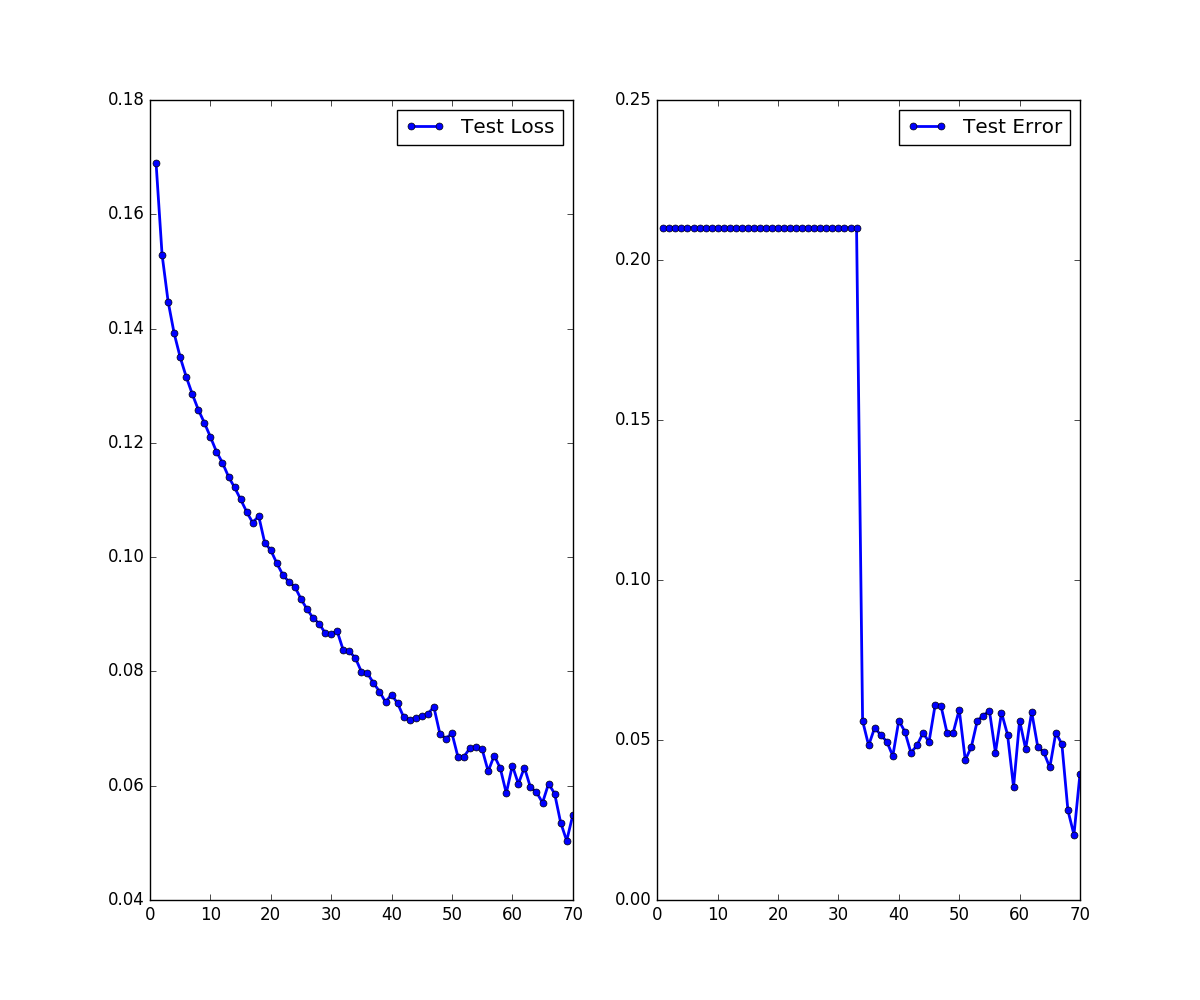
\includegraphics[width=0.95\textwidth]{Test-Statistics-sgd-batchsize=100-mse.png}
\end{minipage}
\end{figure}

In the full batch gradient descent, I run it for 3000 epochs. The results are graphed and tabulated below:
\begin{center}
\begin{tabular}{|c|c|c|}
\hline
& Train Accuracy & Test Accuracy \\
\hline
96 epochs & \(\approx 78.7\%\) & \(\approx 79.4\%\) \\
\hline
3000 epochs & \(94.4\%\) & \(97.99\%\) \\
\hline
\end{tabular}
\end{center}

The variation graph is shown below (L: Train, R: Test):
\begin{figure}[H]
\begin{minipage}{0.49\linewidth}
\centering
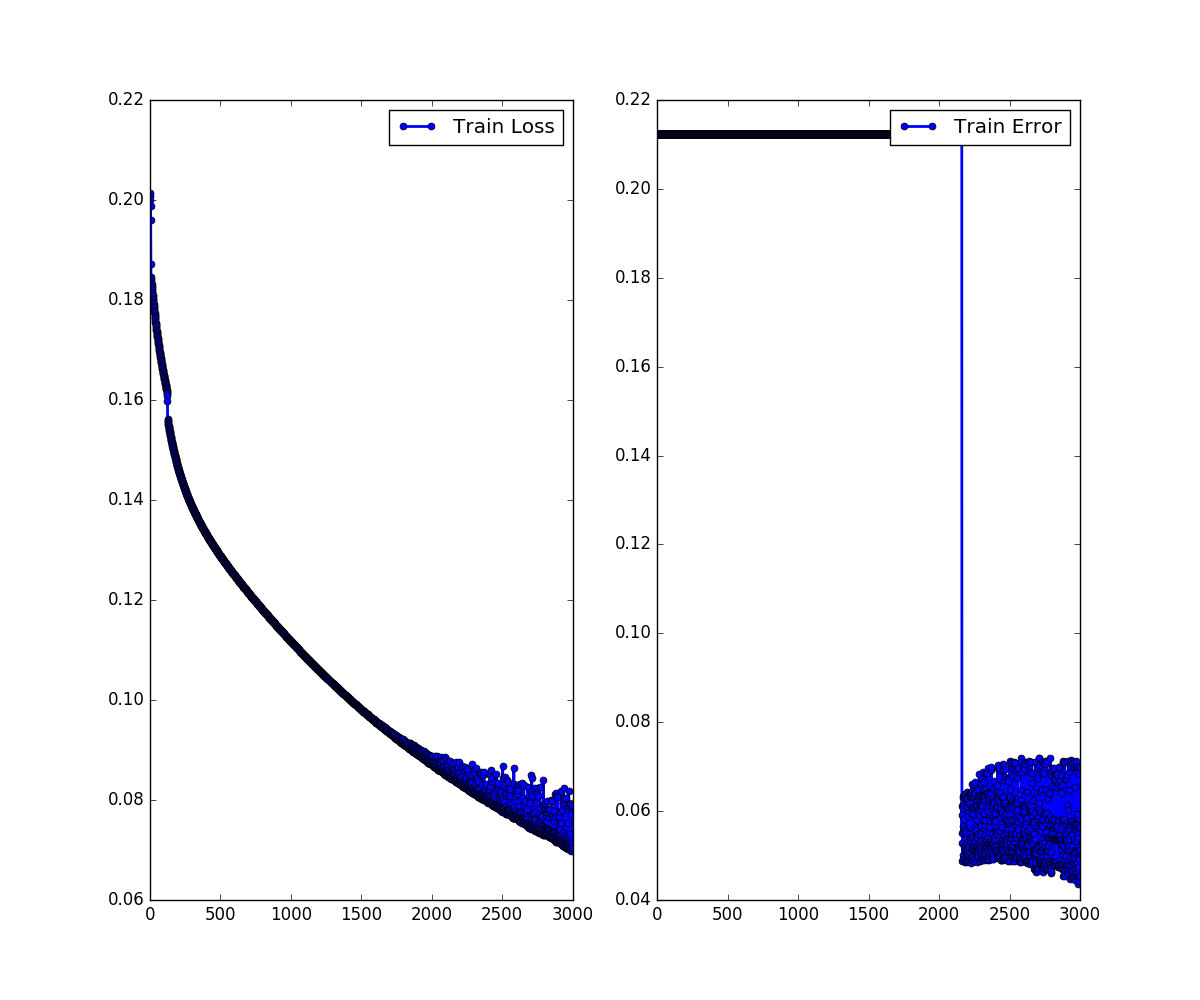
\includegraphics[width=0.95\textwidth]{Train-Statistics-sgd-batchsize=8143-mse.png}
\end{minipage}
\hfill
\begin{minipage}{0.49\linewidth}
\centering
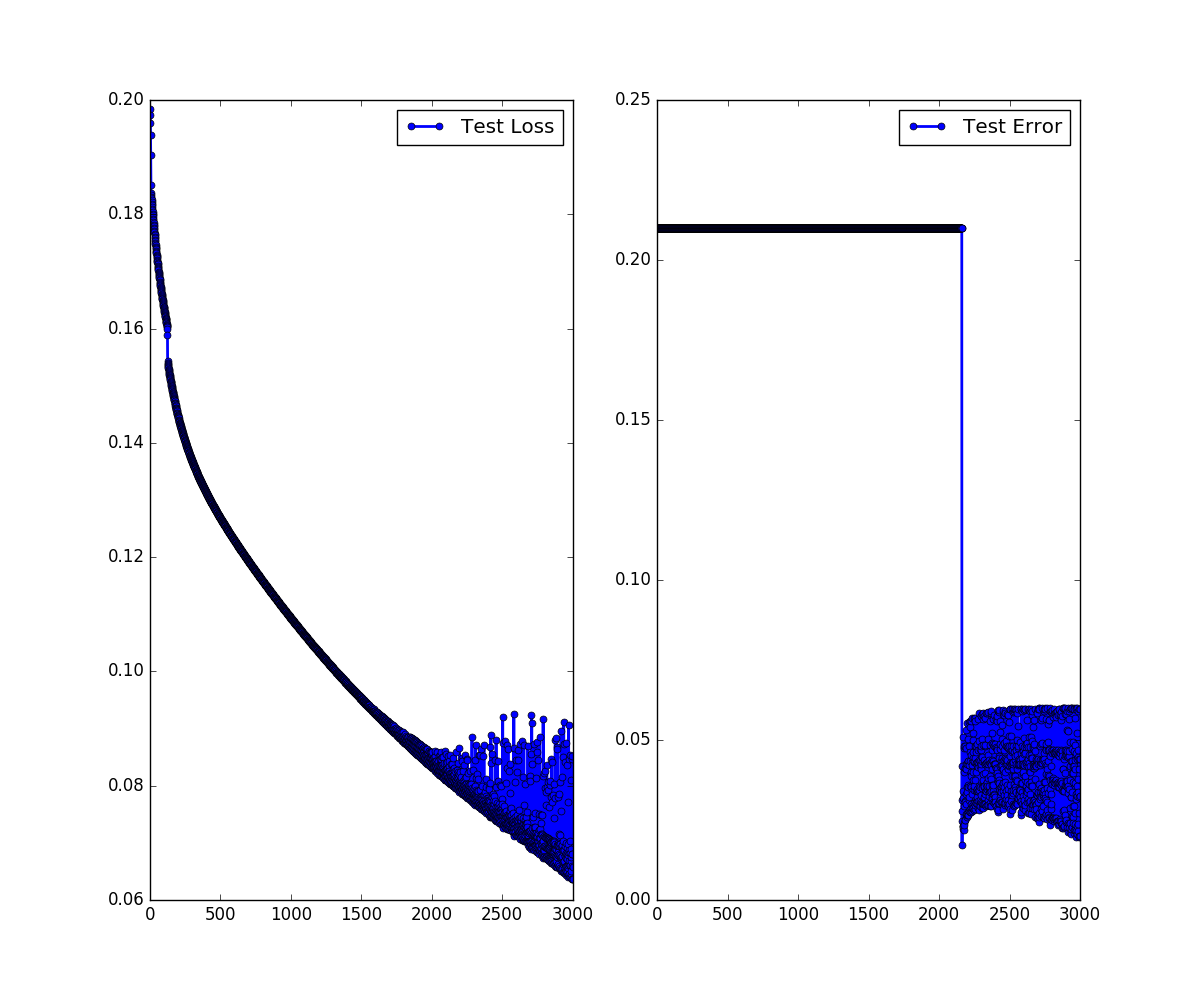
\includegraphics[width=0.95\textwidth]{Test-Statistics-sgd-batchsize=8143-mse.png}
\end{minipage}
\end{figure}

The stopping epochs for the 5 different configurations and the end performance are tabulated below for the analogue of the \textbf{Part e} for the Mean Squared Loss:
\begin{center}
\begin{tabular}{|c|c|c|c|}
\hline
H & Stopping Epochs & Training Set Accuracy & Testing Set Accuracy \\
\hline
1 & 55 & \(\approx 78.8\%\) & \(\approx 79.0\%\)\\
\hline
2 & 290 & \(\approx 98.8\%\)& \(\approx 99.2\%\)\\
\hline
5 & 110 & \(\approx 98.8\%\)& \(\approx 99.2\%\)\\
\hline
10 & 75 & \(\approx 98.8\%\)& \(\approx 99.3\%\)\\
\hline
20 & 65 & \(\approx 98.8\%\)& \(\approx 99.3\%\)\\
\hline
\end{tabular}
\end{center}

Graphically, the variation is shown below (L: Train, R: Test):
\begin{minipage}{0.49\linewidth}
\begin{figure}[H]
\centering
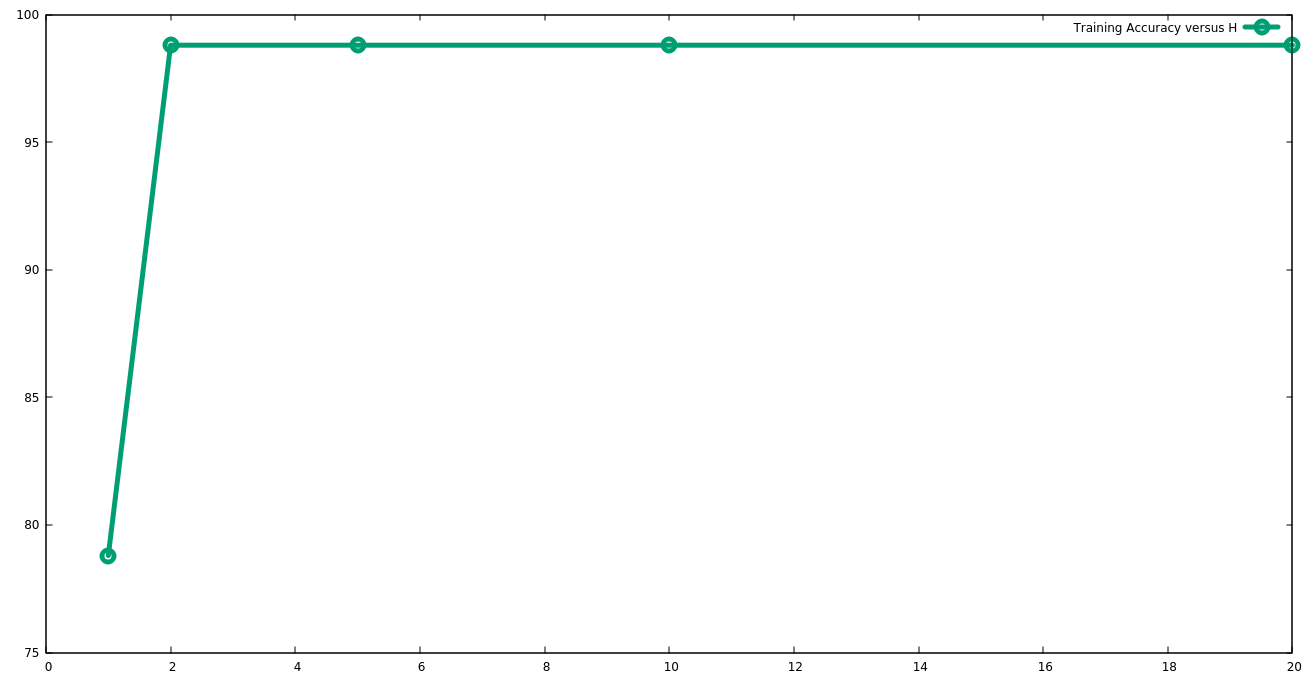
\includegraphics[width=0.95\textwidth]{train_H_MSE.png}
\end{figure}
\end{minipage}
\hfill
\begin{minipage}{0.49\linewidth}
\begin{figure}[H]
\centering
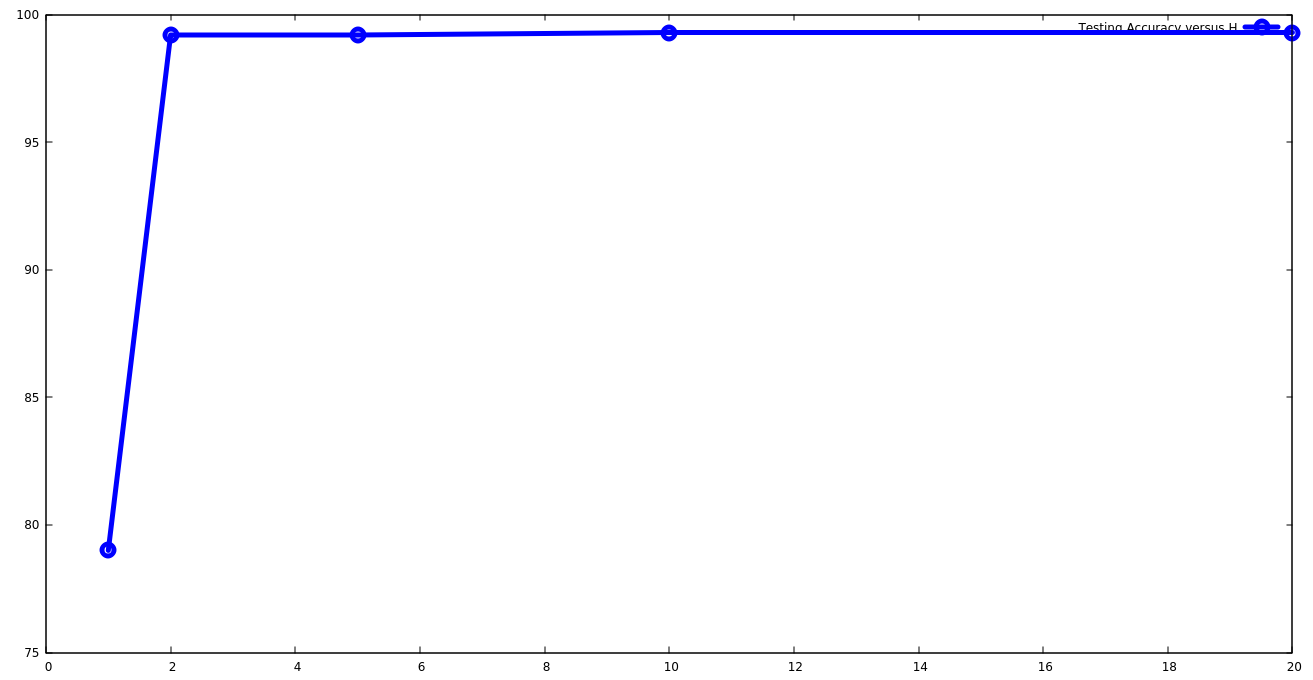
\includegraphics[width=0.95\textwidth]{test_H_MSE.png}
\end{figure}
\end{minipage}
\end{flushleft}

\subsection*{Part g}
\begin{flushleft}
The architecture, epochs trained for and the training and testing accuracies are tabulated below. The loss function is consideration is the binary-cross entropy loss.
\begin{center}
\begin{tabular}{|c|c|c|c|}
\hline
Architecture & Epochs Trained for & Training Accuracy & Testing Accuracy \\
\hline
\texttt{5 - 3 - 2 - 1} & 225 & \(\approx 98.9\%\) & \(\approx 98.1\%\)\\
\hline
\texttt{5 - 2 - 2 - 1} & 225 & \(\approx 98.9\%\) & \(\approx 99.1\%\)\\
\hline
\texttt{5 - 10 - 5 - 1} & 100 & \(\approx 98.9\%\) & \(\approx 98.9\%\)\\
\hline
\texttt{5 - 2 - 3 - 1} & 190 & \(\approx 98.9\%\) & \(\approx 99.1\%\)\\
\hline
\texttt{5 - 10 - 1} & 75 & \(\approx 98.8\%\) & \(\approx 99.2\%\)\\
\hline
\end{tabular}
\end{center}

From the table, it can be seen that multi-hidden-layer neural networks have a (little) better training accuracy than the single layer neural networks. Maybe, because of the over-parameterization, there is a reason of that very small dip in testing accuracy. I use the Adam Optimizer with a global learning rate of \(3 \times 10^{-4}\).
\end{flushleft}
\end{document}
